\chapter{Results and Discussion}

\section{Training Results}

A total of 100,000 games were played for each iteration of model generation. The average loss for each iteration and the wins, draws, and losses against the previous best model for 100 games are shown in Figure \ref{fig:training-results}. A new best model is established when the number of combined wins and draws against the previous best model is greater than or equal to 60 for each iteration.

\pgfplotstableread{
I  W  D L
1  66 0 34
2  53 0 47
3  54 0 46
4  60 0 40
5  59 0 41
6  59 0 41
7  60 0 40
8  48 0 52
9  48 0 52
10 46 0 54
11 56 0 44
12 61 0 39
13 53 0 47
14 49 0 51
15 51 0 49
16 50 0 50
17 51 0 49
18 51 0 49
19 68 0 32
20 49 0 51
}\wdltraindata

\begin{figure}[H]
    \centering
    \begin{subfigure}{0.4\textwidth}
        \centering
        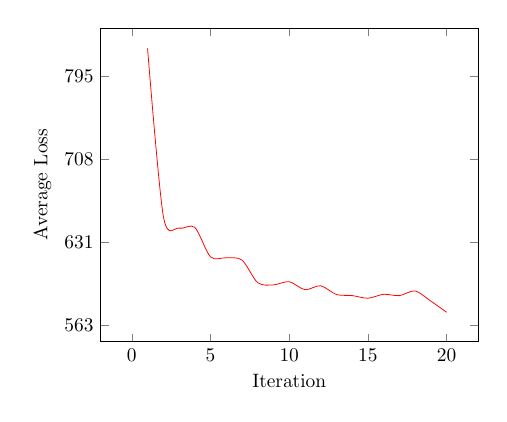
\begin{tikzpicture}[scale=0.7]
          \begin{axis}[
            xmin = -2, xmax = 22,
            ymin = 550, ymax = 850,
            ymode = log, log ticks with fixed point,
            xlabel = Iteration,
            ylabel = Average Loss]
            \addplot[smooth, red] plot coordinates {
                (1 , 826.237610)
                (2 , 654.909119)
                (3 , 644.004456)
                (4 , 644.672119)
                (5 , 618.844055)
                (6 , 618.023010)
                (7 , 616.063965)
                (8 , 597.026978)
                (9 , 595.188477)
                (10, 597.854187)
                (11, 591.271484)
                (12, 594.479980)
                (13, 587.326843)
                (14, 586.461426)
                (15, 584.299072)
                (16, 587.507446)
                (17, 586.405396)
                (18, 590.255615)
                (19, 581.949158)
                (20, 573.042419)
            };
          \end{axis}
        \end{tikzpicture}
        \caption{Average Loss Over Iteration}
        \label{fig:train-loss-per-iteration}
    \end{subfigure}
    \begin{subfigure}{0.4\textwidth}
        \centering
        \begin{tikzpicture}[scale=0.7]
          \begin{axis}[
            ybar stacked,
            bar width=7pt,
            xmin = -2, xmax = 22,
            ymin = 0, ymax = 100,
            xlabel = Iteration]
            \draw (0,60) -- (300,60);
            \addplot[fill=green!50] table [y = W, meta = I] {\wdltraindata};
            \addlegendentry{Win}
            \addplot[fill=blue!50] table [y = D, meta = I] {\wdltraindata};
            \addlegendentry{Draw}
            \addplot[fill=red!50] table [y = L, meta = I] {\wdltraindata};
            \addlegendentry{Loss}
          \end{axis}
        \end{tikzpicture}
        \caption{Win-Draw-Loss Over Iteration}
        \label{fig:train-wdl-per-iteration}
    \end{subfigure}
    \caption{Training Results of the Model Generation}
    \label{fig:training-results}
\end{figure}

As shown in Figure \ref{fig:train-loss-per-iteration}, the average loss of the model continuously got lower as the number of iterations got higher. This shows that the model is learning to accurately predict the WDL probability and the best moves according to the MCTS algorithm of a given state.

Furthermore, the current model of the iteration is pitted against the current best model where the win-draw-loss of the current model against the current best model is shown in Figure \ref{fig:train-wdl-per-iteration}. The models that surpassed 60 combined wins and draws per iteration became the next best model as shown in Table \ref{tab:train-best-models-version-per-iteration}.

\begin{table}[H]
    \centering
    \begin{tabular}{ccc}
        \hline
        Version & Iteration & Wins Against the Previous Version \\ \hline
        v1      & 1         & 66                                \\
        v2      & 4         & 60                                \\
        v3      & 7         & 60                                \\
        v4      & 12        & 61                                \\
        v5      & 19        & 68                                \\ \hline
    \end{tabular}
    \caption{Versions of Trained Best Models and their Iterations}
    \label{tab:train-best-models-version-per-iteration}
\end{table}

The new versions of the best model are better against the previous versions of the best model as shown by the number of wins they got against the previous versions of the best model as shown in Table \ref{tab:train-best-models-version-per-iteration}.

\section{Final Best Model Against Previous Best Models}

The previous versions of the best model were pitted against the final version of the best model for 100 games each with 100 MCTS simulations for each move to assess the competence of the final version of the best model. The wins, draws and losses of the previous best models against the final version of the best model are recorded as shown in Figure \ref{fig:wdl-eval}.

\pgfplotstableread{
V  W  D L
v1 27 0 73
v2 33 0 67
v3 43 0 57
v4 49 0 51
v5 54 0 46
}\wdlevaldata
    
\begin{figure}[H]
    \centering
    \begin{tikzpicture}
      \begin{axis}[
        ybar stacked,
        xtick = data,
        ymin = 0, ymax = 100,
        xtick = data,
        xticklabels from table={\wdlevaldata}{V},
        xlabel = Version]
        \addplot[fill=green!50] table [y = W, meta = V, x expr=\coordindex] {\wdlevaldata};
        \addlegendentry{Win}
        \addplot[fill=blue!50] table [y = D, meta = V, x expr=\coordindex] {\wdlevaldata};
        \addlegendentry{Draw}
        \addplot[fill=red!50] table [y = L, meta = V, x expr=\coordindex] {\wdlevaldata};
        \addlegendentry{Loss}
      \end{axis}
    \end{tikzpicture}
    \caption{Win-Draw-Loss of the Previous Best Models Against the Best Model}
    \label{fig:wdl-eval}
\end{figure}

An increasing trend can be shown in the number of wins that the previous best models makes against the final best model. This trend demonstrates the improvement in competence of the model after the training phase in each iteration. The final best model won 54 games out of 100 competing against itself. According to Mr. Basanes (\textit{personal communications}, May 23, 2025), the first player in the game of Damath has an advantage over the second player as the second player has to catch up with the moves of the first player. The final version of the model wins more than half of the games since a Damath player competing against a player of similar skills and experience may win more if they were the first player and the model evaluation picks a random initial player for the hundred of games played against each evaluation.

\section{Best Model Against an Expert Damath Player}

To analyze the final version of the best model, we let it play against Mr. Basanes for 10 games. He won 7 out of the total games against our best model. Mr. Basanes plays as the red player while the final version of the best model plays as the black player. In this section, the researchers discuss the moves of the final version of the best model that showed strategies worth analyzing according to Mr. Basanes.

% \subsection{First Game Against an Expert Damath Player}

The best model plays first with 500 MCTS simulations for the first game (see Appendix \ref{tab:first-game}) and sets up an elaborate trap by letting Mr. Basanes eat pieces that temporarily gave him an advantage during the first nine moves of the game as shown in Figure \ref{fig:1-9-game1}. The model forced Mr. Basanes to eat the 0 piece, setting up a trap that puts the model in a more advantageous position by having its -11 piece capture the -9 piece of Mr. Basanes that lands on a multiply operator on the eight move.

\begin{figure}[H]
    \centering
    \begin{subfigure}{0.3\textwidth}
        \centering
        \includegraphics[width=\textwidth]{images/games/game1/move_2.png}
        \caption*{Move 1: A = 0 \textbar\ H = 0}
    \end{subfigure}
    \quad
    \begin{subfigure}{0.3\textwidth}
        \centering
        \includegraphics[width=\textwidth]{images/games/game1/move_3.png}
        \caption*{Move 2: A = 0 \textbar\ H = 0}
    \end{subfigure}
    \quad
    \begin{subfigure}{0.3\textwidth}
        \centering
        \includegraphics[width=\textwidth]{images/games/game1/move_4.png}
        \caption*{Move 3: A = 0 \textbar\ H = 0}
    \end{subfigure} \\
    \begin{subfigure}{0.3\textwidth}
        \centering
        \includegraphics[width=\textwidth]{images/games/game1/move_5.png}
        \caption*{Move 4: A = 0 \textbar\ H = -15}
    \end{subfigure}
    \quad
    \begin{subfigure}{0.3\textwidth}
        \centering
        \includegraphics[width=\textwidth]{images/games/game1/move_6.png}
        \caption*{Move 5: A = 0 \textbar\ H = -15}
    \end{subfigure}
    \quad
    \begin{subfigure}{0.3\textwidth}
        \centering
        \includegraphics[width=\textwidth]{images/games/game1/move_7.png}
        \caption*{Move 6: A = 0 \textbar\ H = -27}
    \end{subfigure} \\
    \begin{subfigure}{0.3\textwidth}
        \centering
        \includegraphics[width=\textwidth]{images/games/game1/move_8.png}
        \caption*{Move 7: A = 0 \textbar\ H = 54}
    \end{subfigure}
    \quad
    \begin{subfigure}{0.3\textwidth}
        \centering
        \includegraphics[width=\textwidth]{images/games/game1/move_9.png}
        \caption*{Move 8: A = 0 \textbar\ H = 54}
    \end{subfigure}
    \quad
    \begin{subfigure}{0.3\textwidth}
        \centering
        \includegraphics[width=\textwidth]{images/games/game1/move_10.png}
        \caption*{Move 9: A = 0 \textbar\ H = 45}
    \end{subfigure}
    \caption{First Nine Moves of the First Game Against an Expert Damath Player} % ADVISER COMMENT (DON'T DELETE): need to specify which "game" this 9 moves are from
    \label{fig:1-9-game1}
\end{figure}

This made the model play the tenth move as shown in Figure \ref{fig:10-game1}, which gave the final version of the best model a bigger score compared to Mr. Basanes.

\begin{figure}[H]
    \centering
    \begin{subfigure}{0.3\textwidth}
        \centering
        \includegraphics[width=\textwidth]{images/games/game1/move_11.png}
        \caption*{Move 10: A = 99 \textbar\ H = 45}
    \end{subfigure}
    \caption{Tenth Move of the First Game Against an Expert Damath Player}
    \label{fig:10-game1}
\end{figure}

According to Mr. Basanes (\textit{personal communications}, May 13, 2025), the model uses the same sequence of moves that he discovered to trap players for the first ten moves of the game. The opening sequence of moves that the model played was a solid start to the game of Damath and can lead to eventually winning the game according to Mr. Basanes (\textit{personal communications}, May 13, 2025).

However, Mr. Basanes found a way to gain advantage against the model on the 44th move of the game as shown in Figure \ref{fig:44-46-game1}. Mr. Basanes was able to reverse the situation and eventually win against the best model for the first game. Mr. Basanes made the model capture his 10 dama piece using their -7 piece on a multiply operator, giving the model an added score of -140.

\begin{figure}[H]
    \centering
    \begin{subfigure}{0.3\textwidth}
        \centering
        \includegraphics[width=\textwidth]{images/games/game1/move_45.png}
        \caption*{Move 44: H = 77.5 \textbar\ A = 83.75}
    \end{subfigure}
    \quad
    \begin{subfigure}{0.3\textwidth}
        \centering
        \includegraphics[width=\textwidth]{images/games/game1/move_46.png}
        \caption*{Move 45: H = 77.5 \textbar\ A = 83.75}
    \end{subfigure}
    \quad
    \begin{subfigure}{0.3\textwidth}
        \centering
        \includegraphics[width=\textwidth]{images/games/game1/move_47.png}
        \caption*{Move 46: H = 77.5 \textbar\ A = -56.25}
    \end{subfigure}
    \caption{44th to 46th Moves of the First Game Against an Expert Damath Player}
    \label{fig:44-46-game1}
\end{figure}

% \subsection{Second Game Against an Expert Damath Player}

% For the second game, Mr. Basanes plays first with the best model playing with 500 MCTS simulations. The best model was forced to make his $0$ piece a dama piece in a sequence of moves shown in Figure \ref{fig:6-9-game2}.

% % show how AI's 0 piece became a dama piece
% \begin{figure}[H]
% \centering
%     \begin{subfigure}{0.3\textwidth}
%         \centering
%         \includegraphics[width=\textwidth]{images/games/game2/move_7.png}
%         \caption*{Move 6: H = 77.5 \textbar\ A = 83.75}
%     \end{subfigure}
%     \quad
%     \begin{subfigure}{0.3\textwidth}
%         \centering
%         \includegraphics[width=\textwidth]{images/games/game2/move_8.png}
%         \caption*{Move 7: H = 77.5 \textbar\ A = 83.75}
%     \end{subfigure}
%     \quad
%     \begin{subfigure}{0.3\textwidth}
%         \centering
%         \includegraphics[width=\textwidth]{images/games/game2/move_9.png}
%         \caption*{Move 8: H = 77.5 \textbar\ A = -56.25}
%     \end{subfigure}
%     \begin{subfigure}{0.3\textwidth}
%         \centering
%         \includegraphics[width=\textwidth]{images/games/game2/move_10.png}
%         \caption*{Move 9: H = 77.5 \textbar\ A = -56.25}
%     \end{subfigure}
%     \quad
%     \begin{subfigure}{0.3\textwidth}
%         \centering
%         \includegraphics[width=\textwidth]{images/games/game2/move_11.png}
%         \caption*{Move 9: H = 77.5 \textbar\ A = -56.25}
%     \end{subfigure}
%     \caption{Initial Moves of the Second Game Against an Expert Damath Player}
%     \label{fig:6-9-game2}
% \end{figure}

% Mr. Basanes took advantage of having to capture first, forcing the best model to continuously make capture moves that lessens the score of the best model making him win as shown in Figure.  We suspect that during the self-play data generation \ref{alg:datawgeneration} the model was not able to explore this line of moves, which ultimately led to its loss. 

% \subsection{Third Game Against an Expert Damath Player}

The final version of the best model plays first with 1000 MCTS simulations for the third game (see Appendix \ref{tab:third-game}). Mr. Basanes and the model played the same initial moves as in the first game. After the thirteenth move, the best model made different moves due to the increase in the number of MCTS simulations, letting the best model consider more moves ahead before making a move.

After the 33rd move of the third game, the best model seems to be winning as it has the higher score but the WDL predictions says that Mr. Basanes is most likely to win. However, Mr. Basanes failed to notice other advantageous moves as he said that he was giving more focus to the most active part of the board making him lose as shown in Figure. 

% show the board where WDL is unexpectedly high even though the score is lower then turning low as he played the wrong piece

% add discussions

% After the third game, we let Mr. Basanes go back to the position where the WDL predictions says that he is most likely to win and made him reconsider his moves. After figuring out the best moves to play, he finally won as shown in Figure. % ADVISER COMMENT (DON'T DELETE): remove this result as it is already skewed since Mr. Basanes already lost and this is like giving a "rewind" ability

% show the board where WDL is unexpectedly high even though the score is lower then turning high as he played a good move

% add discussions
